\documentclass[12pt]{report}
\usepackage[a4paper]{geometry}
\usepackage[myheadings]{fullpage}
\usepackage{fancyhdr}
\usepackage{lastpage}
\usepackage{graphicx, wrapfig, subcaption, setspace, booktabs}
\usepackage[T1]{fontenc}
\usepackage[font=small, labelfont=bf]{caption}
\usepackage{fourier}
\usepackage[protrusion=true, expansion=true]{microtype}
\usepackage[english]{babel}
\usepackage{sectsty}
\usepackage{listings}
\usepackage{xcolor}
\usepackage{mathtools}
\usepackage[cc]{titlepic}
\usepackage{graphicx}



\newcommand{\HRule}[1]{\rule{\linewidth}{#1}}
\onehalfspacing
\setcounter{tocdepth}{5}
\setcounter{secnumdepth}{5}


%New colors defined below
\definecolor{codegreen}{rgb}{0,0.6,0}
\definecolor{codegray}{rgb}{0.5,0.5,0.5}
\definecolor{codepurple}{rgb}{0.58,0,0.82}
\definecolor{backcolour}{rgb}{0.95,0.95,0.92}

%Code listing style named "mystyle"
\lstdefinestyle{mystyle}{
  backgroundcolor=\color{backcolour}, commentstyle=\color{codegreen},
  keywordstyle=\color{magenta},
  numberstyle=\tiny\color{codegray},
  stringstyle=\color{codepurple},
  basicstyle=\ttfamily\footnotesize,
  breakatwhitespace=false,         
  breaklines=true,                 
  captionpos=b,                    
  keepspaces=true,                 
  numbers=left,                    
  numbersep=5pt,                  
  showspaces=false,                
  showstringspaces=false,
  showtabs=false,                  
  tabsize=2
}

%"mystyle" code listing set
\lstset{style=mystyle}



%-------------------------------------------------------------------------------
% HEADER & FOOTER
%-------------------------------------------------------------------------------
\pagestyle{fancy}
\fancyhf{}
\setlength\headheight{15pt}
\fancyfoot[R]{Page \thepage\ of \pageref{LastPage}}


%-------------------------------------------------------------------------------
% TITLE PAGE
%-------------------------------------------------------------------------------
\begin{document}

\title{ \begin{center}
    Summer of Science 2021
        \end{center}
        \HRule{0.5pt} \\
		\LARGE \textbf{\uppercase{Data Mining}}
		\HRule{2pt} \\
		\normalsize \today \vspace*{5\baselineskip}}

\date{}

\titlepic{
\includegraphics[width=0.8\textwidth]{images/data-mining-definition.jpg}}


\author{
		Aniket Pokle \\ 
		Mentor: Deepanshu Bagotia \\
		}


\maketitle
\tableofcontents
\newpage

%-------------------------------------------------------------------------------
% Section title formatting
\sectionfont{\scshape}
%-------------------------------------------------------------------------------
\section*{Introduction}
\addcontentsline{toc}{section}{Introduction}
\fancyhead[R]{Introduction}

Data mining is a process of extracting and discovering patterns in large data sets involving methods at the intersection of machine learning, statistics, and database systems. Data mining is an interdisciplinary subfield of computer science and statistics with an overall goal to extract information (with intelligent methods) from a data set and transform the information into a comprehensible structure for further use. Data mining is the analysis step of the "knowledge discovery in databases" process, or KDD. Aside from the raw analysis step, it also involves database and data management aspects, data pre-processing, model and inference considerations, interestingness metrics, complexity considerations, post-processing of discovered structures, visualization, and online updating.\\
\\
The term "data mining" is a misnomer, because the goal is the extraction of patterns and knowledge from large amounts of data, not the extraction (mining) of data itself.\\
\\
While data analysis is used to test models and hypotheses on the datasets, data mining on the other hand uses machine learning and statistical models to uncover clandestine or hidden patterns in a large volume of data.\\
\\
In this report I try to understand some of the statistical and machine learning aspects of Data mining such as data management using SQL, data pre{-}processing, model and inference considerations and machine learning algorithms used in data mining.
\newpage
\section*{PROBABILITY AND STATISTICS}
\addcontentsline{toc}{section}{Probability and Statistics}
\fancyhead[R]{PROBABILITY AND STATISTICS}

\subsection*{Probability}
The extent to which an event is likely to occur, measured by the ratio of the favourable cases to the
whole number of cases possible.\\
Basically Probability is the measure of uncertainity.

\subsection*{Sample space and Event}
Any activity for which the outcome is uncertain can be thought of
as an “experiment.”\\
The set of all possible outcomes of an experiment is known as the
sample space of the experiment and is denoted by $\Omega$.\\
Any subset E of the sample space is known as an event.\\
An event is a set of possible outcomes of the experiment.

\subsection*{Baye's Theorem}
Bayes Theorem provides a principled way for calculating a conditional probability.\\
$Assume\ that\ A_1,A_2,...A_m\ are\ events\ such\ that$
\begin{itemize}
    \item $A_1 \cup A_2 \cup ...\cup A_m = \Omega $
    \item $A_i \cap A_j = \phi \ (pairwise disjoint)\ \forall i \neq j = 1,2,...m$
    \item $P(A_i) > 0 \ for \ all \ i \ and \ B \ is \ another \ event \ than \ A, \ then$
\end{itemize}
\[
P(A_i|B) = \frac{P(B|A_j)P(A_j)}{\sum_{i=1}^{m}P(B|A_i)P(A_i)}
\]
is known as Bayes' Formula\\
$P(A_i) : Prior\ probabilities$\\
$P(A_i|B) : Posterior\ probabilities$\\
$P(B|A_i) : Model\ probabilities$

\subsection*{Independent Events}
\textbf{Definition}: Two random events A and B are called (stochastically)
independent If P(AB) = P(A) P(B).\\
i.e. if the probability of simultaneous occurrence of both events A
and B is the product of the individual probabilities of occurrence of A
and B.

\subsection*{Need of Random Variable}
In any random experiment, we are interested in the value of some
numerical quantity determined by the result.\\
We are not interested in all the details of the experiments.\\
These quantities of interest that are determined by the result of the
experiment are known as random variables.

\subsection*{Random Variable}
Let $\Omega$ represent the sample space of a random experiment, and
let R be the set of real numbers.\\
A random variable is a function X which assigns to each element
$\omega \in \Omega$ one and only one number
\[ X(\omega) = x, x \in R,\ i.e.\ X : \Omega \rightarrow R \]

\subsection*{Probability Density Function(PDF) for Continuous Random Variable}
For a function f(X) to be a probability density function (PDF) of a
continuous random variable X, it needs to satisfy the following
conditions:
\begin{enumerate}
    \item f(X) $\leq 0 \forall x \in R$ 
    \item $\int_{-\infty}^{\infty}f(x)\ dx \ = \ 1$
\end{enumerate}
Let X be a random variable with CDF F(x).\\
If $x_1\ <\ x_2$ where $x_1\ and\ x_2$ are known constants,
\[ P(x_1 \leq X \leq x_2) = F(x_2)\ -\ F(x_2)\ = x_2\ -\ x_1\ =\ \int_{x_1}^{x_2}f(x)\ dx\]


\subsection*{Cumulative Distribution Function(CDF)}
The cumulative distribution function, or more simply the distribution
function, F of the random variable X is defined for any real number x
by
\[F(x) = P(X \leq x)\]
That is, F(x) is the probability that the random variable X takes on a
value that is less than or equal to x.

\subsection*{CDF of Continuous Random Variables}
A random variable X is said to be continuous if there is a function
f(x) such that for all x $\in$ R
\[ F(x)\ =\ \int_{-\infty}^{\infty}f(t)\ dt \]
holds.
\begin{itemize}
    \item F(x) is the CDF of X, and
    \item f(x) is the PDF of X.
\end{itemize}

\subsection*{CDF of Discrete Random Variable}
The cumulative distribution function CDF of a discrete random
variable as
\[ F(X)\ =\ \sum_{i=1}^{k} I_{x_i \leq x}p_i \]
where I is an indicator function defined as
\begin{equation}
I_{x_i \leq x} = 
\begin{cases}
&1\ if\ x_i \leq x\\
&0\ otherwise.
\end{cases}
\end{equation}
The CDF of a discrete variable is always a step function.



\subsection*{Expectation of a Continuous Random Variable}
Let X be a continuous random variable having the probability
density function f (x).\\
Suppose g(X) is a real valued function of X.\\
Obviously g(X) will also be a random variable.\\
Then expectation of g(X) is defined as is defined as
\[ E[g(X)]\ =\ \int_{-\infty}^{\infty} g(x)f(x)\ dx \]
provided with \[ \int |g(x)|f(x)\ dx < \infty \]

\subsection*{Expectation of a Discrete Random Variable}
Let X be a discrete random variable having the probability mass
function P(X = $x_i$) = $p_i$ .
Suppose g(X) is a real valued function of X.
Obviously g(X) will also be a random variable.
Thus X takes the values $x_1, x_2,...,x_k$ with respective
probabilities $p_1, p_2, . . ., p_k $
Then expectation of g(X) exists and is defined as
\[ E[g(X)]\ =\ \sum_{i=1}^{\infty} g(x_i)P(X\ =\ x_i)\ =\ \sum_{i=1}^{\infty} g(x_i)p_i \]
provided \[ \sum_{i=1}^{\infty} |g(x_i)|p_i < \infty \]

\subsection*{Moments}
Moments are used to describe different characteristics and
features of a probability distribution, viz., central tendency,
disperson, symmetry and peakedness (hump) of probability curve.
\begin{enumerate}
    \item g(X) = $X^r$ where r is nonnegative integer,\\
    then E[g(X)] = E($X^r$) = $\mu_r^`$\\
    $\mu_r^`$ is called as the $r^{th}$ moment of X about origin.
    \item g(X) = $(X - A)^r$ where r is non{-}negative integer,\\
    then E[g(X)] = E$(X - A)^r$\\
    is called as $r^{th}$ moment of X about the point "A".
\end{enumerate}

\subsection*{Central Moment}
The moments of a variable X about the arithmetic mean $\bar x$ are
called central moments.\\
For  E[g(X)] = E$(X - A)^r$\\
If A = E(X) : Mean \\
then E$(X - A)^r$ = $E[X\ -\ E(X)]^r$ = $\mu_r$\\
$\mu_r$ is called as the $r^{th}$ central moment of X.

\subsection*{Quantiles}
We define quantiles in terms of the distribution function.\\
The value $x_p$ for which the cumulative distribution function is\\
F($x_p$) = p (0 $\leq$ p $\leq$ 1)\\
is called the p‐quantile.\\
$x_p$ is the value which divides the CDF into two parts:
\begin{itemize}
    \item the probability of observing a value left of $x_p$ is p
    \item the probability of observing a value right of $x_p$ is 1 - p.
\end{itemize}

\subsection*{Tschebyschev's Inequality}
If we do not know the distribution of a random variable X, we can still
make statements about the probability using Tschebyschev’s
inequality that X takes values in a certain interval (which has to be
symmetric around the expectation $\mu$) if the mean $\mu$ and the variance
$\sigma^2$ of X are known.\\
Let X be a random variable with E(X) = $\mu$ and Var(X) = $\sigma^2$. It holds that \[ P(|X\ -\ \mu| \geq \ c)\ \leq \ \frac{Var(X)}{c^2} \]
This is equivalent to \[ P(|X\ -\ \mu|\ <\ c)\ \leq \ 1\ -\ \frac{Var(X)}{c^2} \]

\subsection*{Need of Probability Distributions}
Probability distribution functions have
special properties and describe how probabilities are distributed
under different conditions.\\
The form of such functions depends upon the nature and complexity
of the phenomenon under consideration.\\
We have probability distributions for discrete and continuous
random variables.

\subsection*{Degenerate Distribution}
A random variable X has a degenerate distribution at c, if c is the only
possible outcome.\\
The probability mass function (PMF) of X is given by
\begin{equation}
P(X = x) =
\begin{cases}
& $1\ if\ x\ =\ c$\\
& 0\ if\ x\ \neq \ c
\end{cases}
\end{equation}

The CDF in such case is given by
\begin{equation}
F(X) = 
\begin{cases}
&$0\ if\ x\ <\ c$\\
&1\ if\ x\ \geq \ c.
\end{cases}
\end{equation}
Further, The mean (expectation) and variance of X are \textbf{E(X) = c}
and \textbf{Var(X) = 0}.\\
The degenerate distribution indicates that there is only one possible
fixed outcome, and therefore, no randomness is involved.

\subsection*{Discrete Uniform Distribution}
Consider a situation where the probability of all the outcomes are
the same.\\
In such situations, the discrete uniform distribution can be used to
describe the probabilities and the phenomenon.\\
The discrete uniform distribution assumes that all possible outcomes
have equal probability of occurrence.
\subsubsection*{PMF}
A discrete random variable X with k possible outcomes $x_1, x_2, . . . ,x_k$
is said to follow a discrete uniform distribution if the probability
mass function (PMF) of X is given by
\[ P(X = x_i) = \frac{1}{k} \ \forall \ i\ =\ 1,2,...k.\]
\subsubsection*{Mean and Variance}
If the outcomes are the natural numbers $x_i$ = i (i = 1, 2, . . . , k), then
the mean and variance of X are as follows:
\[ E(X)\ =\ \frac{k+1}{2} \]
\[ Var(X)\ =\ \frac{k^2\ -\ 1}{2} \]

\subsection*{Bernoulli Distribution}
A Bernoulli experiment is a random experiment, the outcome of
which can be classified in but one of two mutually exclusive and
exhaustive ways, e.g. success or failure.\\
If we let X = 1 when the outcome is a success and X = 0 when it is a
failure, then a random variable X has a Bernoulli distribution if the
probability mass function (PMF) of X is given by
\begin{equation}
P(X\ =\ x)\ = 
    \begin{cases}
    & p\; if\ x\ =\ 1\\
    & 1\ -\ p\; if\ x\ =\ 0.
    \end{cases}
\end{equation}
The CDF in such case is given by
\begin{equation}
F(X)\ =
    \begin{cases}
    & 0\; if\ x\ <\ 0\\
    &1\ -\ p\; if\ 0\ \leq \ x \ \leq\ 1 \\
    &1\; if\ x\ \leq\ 1.
    \end{cases}
\end{equation}
The mean(expectation) and variance of a Bernoulli random variable are calculated as \textbf{E(X) = p} and \textbf{Var(X) = p(1 – p)}.

\subsection*{Binomial Distribution}
Consider n independent trials or repetitions of a Bernoulli
experiment with probability of success p in each trial so that p
remains constant in each trial.\\
In each trial or repetition, we may observe either A or $\bar{A}$.\\
At the end of the experiment, we have thus observed A between 0
and n times.\\
Suppose we are interested in the probability of A occurring k times,
then the binomial distribution is useful.\\
A discrete random variable X is said to follow a binomial distribution
with parameters n and p if its PMF is given by
\begin{equation}
P(X = k) =
    \begin{cases}
    & \binom{n}{k}p^k\ q^{n-k}\ if\ k\ =\ 0,1,...n\\
    & 0\ otherwise.
    \end{cases}
\end{equation}
We also write X ~ B(n,p).\\
The mean and variance of a binomial random variable X are given by \textbf{E(X) = np}, \textbf{Var(X) = np(1 - p)}.\\
\textbf{Remark}: A Bernoulli random variable is therefore B(1, p) distributed.

\subsection*{Poisson Distribution}
A discrete random variable X is said to follow a Poisson distribution
with parameter $\lambda$ > 0 if its PMF is given by
\[ P(X = x)\ =\ \frac{\lambda^x\ exp(-\lambda)}{x!}\   x\ =\ 0,1,2,..\]
We also write X ~ P($\lambda$).\\
The mean and variance of a Poisson random variable are identical:
E(X) = Var(X) = $\lambda$

\subsection*{Geometric Distribution}
The geometric distribution can be used to determine the probability
that the event of interest happens at the $k^{th}$ trial for the first time.\\
A discrete random variable X is said to follow a geometric distribution
with parameter p if its PMF is given by
\[ P(X = k)\ =\ p(1-p)^{k-1},\ k\ =\ 1,2,3,...\]
The mean (expectation) and variance are given by
\[ E(X)\ =\ \frac{1}{p}\]
\[ Var(X)\ =\ \frac{1-p}{p^2} \] 

\subsection*{Continuous Uniform Distribution}
A continuous random variable X is said to follow a (continuous)
uniform distribution in the interval [a, b], if its probability density
function (PDF) is given by
\begin{equation}
f_x(x) \equiv f(x) =
\begin{cases}
& \frac{1}{b-a}\ if\ a\ \leq\ x\ \leq\ b,\ (a<b)\\
& 0\ otherwise.
\end{cases}
\end{equation}
We also write X ~ U(a,b).\\
The mean and variance of a X ~ U(a,b) are given by
\[ E(X)\ =\ \frac{a+b}{2}\]
\[ Var(X)\ =\ \frac{(b-a)^2}{12} \] 

\subsection*{Normal Distribution}
The normal distribution is also often called a \textbf{Gaussian distribution}.\\
The most widely used model for the distribution of a random
variable is a normal distribution.\\
A random variable X is said to follow a normal distribution with
parameters $\mu$ and $\sigma^2$ if its PDF is given by
\begin{equation}
    f(x;\mu,\sigma^2)\ \equiv\ f(x)\ =\ \frac{1}{\sigma\sqrt{2\pi}}exp(\frac{-(x-\mu)^2}{2\sigma^2}) \\
    -\infty\ <\ x\ <\ \infty;\ -\infty\ <\ \mu\ <\ \infty;\ \sigma^2\ >\ 0.
\end{equation}
We write X ~ N($\mu$,$\sigma^2$).\\
The mean and variance of X are \textbf{E(X) = $\mu$} and \textbf{Var(X) = $\sigma^2$} respectively.\\
The value of E(X) = $\mu$ determines the center of the probability density function and the value of Var(X) = $\sigma^2$ determines the width.
\subsubsection*{Standard Normal Distribution}
If $\mu$ = 0 and $\sigma^2$ = 1, then X is said to follow a standard normal distribution.\\
We write X ~ N(0,1).

\subsection*{Exponential Distribution}
The exponential distribution is useful in many situations, for example
when one is interested in the waiting time, or lifetime, until an event
of interest occurs.\\
A continuous random variable X is said to follow an exponential
distribution with parameter $\lambda$ > 0, if its probability density function
(PDF) is given by
\begin{equation}
    f_x(x)\ \equiv\ f(x)\ =\
    \begin{cases}
    & \lambda exp(-\lambda x),\ \ if\ 0\ \leq\ x\ \leq\ \infty\\
    & 0\ \ otherwise
    \end{cases}
\end{equation}
We also write X ~ Exp($\lambda$).\\
The mean and variance of X are 
\[ E(X)\ =\ \frac{1}{\lambda}\]
\[ Var(X)\ =\ \frac{1}{\lambda^2}\]
respectively.\\
The CDF of exponential distribution is given as
\begin{equation}
    F(x)\ =\
    \begin{cases}
    & 1\ -\ exp(-\lambda x),\ \ if\ 0\ \leq\ x\ \leq\ \infty\\
    & 0\ \ otherwise
    \end{cases}
\end{equation}

\subsection*{Joint Probability Distributions}
If X and Y are discrete random variables, the joint probability
distribution of X and Y is a description of the set of points (x, y) in the
range of (X, Y) along with the probability of each point.\\
The joint probability distribution of two random variables is referred
to as the bivariate probability distribution or bivariate distribution of
the random variables.
\subsubsection*{Discrete Random Variables}
The joint probability mass function of the discrete random variables
X and Y, denoted as $p_{XY}$(x, y), satisfies
\begin{itemize}
    \item $p_{XY}$(x, y) $\geq$ 0
    \item $\sum_{x}\sum_{y}p_{XY}$(x, y) = 1
    \item p(x,y) = P(X=x, Y=y)
\end{itemize}
\subsubsection*{Continuous Random Variables}
The joint probability distribution of two continuous random
variables X and Y can be specified by providing a method for
calculating the probability that X and Y assume a value in any region
R of two‐dimensional space.\\
Analogous to the probability density function of a single continuous
random variable, a joint probability density function can be defined
over two‐dimensional space.
\subsection*{Joint Cumulative Distribution Function}
A bivariate random variable (X, Y) is continuous if there is a function
$f_{XY}$(x, y) such that
\[ F_{XY}(x,y)\ =\ P(X\leq x,\ Y\leq y)\ =\ \int_{-\infty}^{y}\int_{-\infty}^{x}f_{XY}(x,y)\ dxdy \]
holds.\\
The function $F_XY$(x, y) is the joint cumulative distribution function of
X and Y.

\subsection*{Covariance}
The covariance between X and Y is defined as\\
Cov(X, Y) = E[(X - E(X))(Y - E(Y))] = E(XY) - E(X) E(Y).\\
This is based on Product and first moments.\\
The covariance is
\begin{itemize}
    \item positive if, on average, larger values of X correspond to larger
values of Y
    \item it is negative if, on average, greater values of X correspond to
smaller values of Y.
\end{itemize}
If the random variables $X_1$ and $X_2$ are bivariate, the covariance
matrix is defined as
\[
Cov\binom{X_1}{X_2}\ =\ \binom{Var(X_1)\ \ \ \ Cov(X_1,X_2)}{Cov(X_1,X_2)\ \ \ Var(X_2)}
\]
Also Note that Cov($X_1$,$X_2$) = Cov($X_2$,$X_1$)

\subsection*{Bivariate Normal Distribution}
An extension of a normal distribution to two random variables is
bivariate normal distribution.\\
An extension of a normal distribution to more than two random
variables is multivariate normal distribution.\\
The probability density function of a bivariate normal distribution is
\[
f_{XY}(x,y,\sigma_x,\sigma_y,\mu_x,\mu_y,\rho)\ =\]
\[
\frac{1}{2\pi\sigma_x\sigma_y\sqrt{1-p^2}}exp\Bigg\{-\frac{1}{2(1-p^2)}\left[\frac{(x-\mu_x)^2}{\sigma_x^2}\ +\ \frac{(y-\mu_y)^2}{\sigma_y^2}\ -\ \frac{2\rho(x-\mu_x)(y-\mu_y)}{\sigma_x\sigma_y}\right]\Bigg\}
\]
\[
-\infty\ <\ x\ <\ \infty,\ -\infty\ <\ y\ <\ \infty,\ \sigma_x\ >\ 0,\ \sigma_y\ >\ 0, -1\ <\ \rho <\ 1.
\]

\subsection*{Chi square($\chi^2$) Distribution}
Let $Z_1, Z_2,..., Z_n$ be n independent and identically N(0,1){-}distributed
random variables. The sum of their squares, $\sum_{i=1}^{n}Z_i^2$ is then $\chi^2$ distributed with n degrees of freedom and is denoted as $\chi_n^2$\\
A random variable X has a $\chi_n-$ distribution if the PDF of X is given as
\[
f(x)\ =\ 
\begin{cases}
& \frac{x^{\frac{n-2}{2}}exp(\frac{-x}{2})}{2^{\frac{n}{2}}\Gamma\binom{n}{2}},\ x\ >\ 0 \\
& 0\ otherwise
\end{cases}
\]
We write X ~ $\chi_n^2$.\\
The mean and variance of a random variable $\chi_n^2$ distribution is \\
E(X) = n\\
Var(X) = 2n   respectively.\\
The $\chi_n^2$ distribution is not symmetric.\\
A $\chi_n^2$ distributed random variable can only realize values greater than
or equal to zero.

\subsection*{t {-} Distribution}
Let X and Y be two independent random variables where X ~ N(0,1)
and Y ~ $\chi_n^2$. Then the ratio
\[ \frac{X}{\sqrt{\frac{Y}{n}}}\ \simeq\ t_n \]
follows a t \- distribution (Student's t\-distribution) with degree n of freedom. This is central t\-distribution.\\
A random variable X has a t{-}distribution if the PDF of X is given as
\[
f(x)\ =\ \frac{\Gamma\frac{n+1}{2}}{\sqrt{n\pi}\Gamma\binom{n}{2}}\Bigg(1\ +\ \frac{x^2}{n}\Bigg)^\frac{-n-1}{2}\ \ ; -\infty\ <\ x\ <\ \infty.
\]
The mean and variance of a random variable X ~ $t_n$ distribution is \\
E(X) = 0, n > 1\\
Var(X) = $\frac{n}{n-2}$, n > 2  respectively.\\
The t\-distribution is a symmetric distribution.

\subsection*{F {-} Distribution}
Let X and Y be two independent random variables where X ` $\chi_m^2$
and Y ~ $\chi_n^2$ . Then the ratio
\[ \frac{\frac{X}{m}}{\frac{Y}{n}}\ \simeq\ F_{m,n} \]
follows the Fisher F{-}distribution with (m, n) degrees of freedom. We
write X ~ $F_{m,n}$.\\
The mean and variance of a random variable X ~ $F_{m,n}$ distribution is\\
\[E(X)\ =\ \frac{n}{n-2},\ n\ >\ 2\]
\[Var(X)\ =\ \frac{2n^2(m+n-2)}{m(n-2)^2(n-4)},\ n\ >\ 4\]
respectively.\\
The F random variable is non\-negative, and the distribution is skewed to the right.\\
The “degrees of freedom” specify the shape of the distribution.

\subsection*{Weak Law of Large Numbers}
A positive integer n can be determined such that if a random sample
of size n or larger is taken from a population with the density f(x)
(with E(X) = $\mu$), the probability can be made to be as close to 1 as
desired that the sample mean $\bar{X}$ will deviate from $\mu$ by less than any arbitrarily specified small quantity.
If n is any integer greater than $\frac{\sigma^2}{\epsilon\delta^2}$, then
\[ P[|\bar{X_n}\ -\ \mu|\ <\ \epsilon]\ \geq\ 1\ -\ \delta \]
where $\epsilon$ > 0 and 0 < $\delta$ < 1.

\subsection*{Central Limit Theorem}
The central limit theorem tells that the sum of
a large number of independent random variables has approximately
a normal distribution.\\
It provides a simple method for computing approximate probabilities
for sums of independent random variables
\subsubsection*{Theorem}
Let $X_1, X_2,..., X_n$ be a sequence of independent and identically
distributed random variables each having mean $\mu$ and variance $\sigma^2$ .\\
Then for n large, the distribution of $X_1\ +\ X_2\ +\ ,..., X_n$ is approximately
normal with mean $n\mu$ and variance $n\sigma^2$.\\
It follows from the central limit theorem that
\[ \frac{X_1\ +\ X_2\ +\ ,..., X_n\ -\ n\mu}{\sigma\sqrt{n}} \]
is approximately normal with mean 0 and variance 1, i.e. Standard
normal distribution N(0, 1).

\subsubsection*{Continuity Correction}
When we approximate the probabilities for discrete distributions,
we incorporate the continuity correction also.\\
Let $X_1\ +\ X_2\ +\ ,..., X_n$ be a sequence of independent and identically distributed discrete random variables and let
\[ Y\ =\ X_1\ +\ X_2\ +\ ,..., X_n\]
Suppose that we are interested in finding P(A) = P(l$\leq$Y$\leq$u) using the CLT, where l and u are integers. Since Y is an integer{-}valued random variable, we can write
\[
P(A)\ =\ P\Bigg(l\ -\ \frac{1}{2}\ \leq\ Y\ \leq\ u\ +\ \frac{1}{2}\Bigg)
\]
It turns out that the above expression sometimes provides a better approximation for P(A) when applying the CLT. This is called the continuity correction and it is particularly useful when Y is binomial.

\subsection*{Sample Mean Distribution}
Let $X_1\ +\ X_2\ +\ ,..., X_n$ be a sample from a population having mean $\mu$ and variance $\sigma^2$. The central limit theorem can be used to approximate the distribution of the sample mean
$\bar{X_n}\ =\ \frac{1}{n}\sum_{i=1}^{n}X_i$.\\
Since E($\bar{X_n}$) = $\mu$, Var($\bar{X_n}$) = $\frac{\sigma^2}{n}$ and $\bar{X_n}$ is based on a linear combination of normally distributed random variables, so when sample size n is large, then
\[ \frac{\bar{X_n}\ -\ \mu}{\frac{\sigma}{\sqrt{n}}} \]
has approx. a standard normal distribution N(0,1).

\subsection*{Statistical Inference}
After completing the experiment, data is described and
summarized with an aim to draw a statistical conclusion using the
tools of inferential statistics.\\
A careful description and presentation of the data enable us to
infer an appropriate probability model for a given data set which
can be verified by using the additional data.\\
The tools of statistical inference lay the foundation of the
formulation of a probability model to describe the data.

\subsection*{Unbiased Estimators}
An estimator should be “close” in some sense to the true value of
the unknown parameter.\\
Formally, we say that $\hat{\theta}$ is an unbiased estimator of $\theta$ if the expected value of $\hat{\theta}$ is equal to $\theta$.\\
This is equivalent to saying that the mean of the probability
distribution of (or the mean of the sampling distribution of) $\hat{\theta}$ is equal to $\theta$.

\subsection*{Efficiency of Estimators}
Let the parametric space of $\theta$ be $\Theta$, i.e. $\theta \ \in \  \Theta$.\\
Let $\hat{\theta_1}$ and $\hat{\theta_2}$ be the unbiased estimators of ${\theta}$.\\
Then $\hat{\theta_1}$ is said to be more efficient than $\hat{\theta_2}$ under the variance criterion for estimating $\theta$ when 
\[
Var(\hat{\theta_1})\ \leq\ Var(\hat{\theta_2})\ \forall\ \theta\ \in \ \Theta\]
and
\[
Var(\hat{\theta_1})\ <\ Var(\hat{\theta_2})\ for\ at\ least\ one \theta\ \in \ \Theta\]

\subsection*{Cramer{-}Rao Lower Bound(CRLB)}
Let $X_1,X_2,...,X_n$ is a random sample from a distribution with f(x;$\theta$) $\in$ $\Theta$ and g($\theta$) is to be estimated.\\
CRLB provides a lower bound for the variance of any unbaised estimator of g($\theta$).

\subsection*{Consistency of Estimators}
For a good estimator, as the sample size increases, the values of the
estimator should get closer to the parameter being estimated.\\
This property of estimators is referred to as consistency.

\subsection*{Sufficiency of Estimators}
\subsubsection*{Definition}
Let $X_1,X_2,...,X_n$ be a random sample from a
probability density function (or probability mass function) $f_x(x,\theta)$.\\
A statistic T is said to be sufficient for $\theta$ if the conditional
distribution of $X_1,X_2,...,X_n$ given T = t is independent of $\theta$.\\
\textbf{Note:} This method does not give a constructive way to find out a sufficient statistic. It can only verify if a statistic is sufficient or not.
\subsubsection*{Neyman{-}Fisher Factorization Theorem}
Let $X_1,X_2,...,X_n$ be a random sample from a
probability density function (or probability mass function) $f_x(x,\theta)$.\\
A statistic T = $T(x_1,x_2,...,x_n)$ is said to be sufficient for $\theta$ iff the joint density of $X_1,X_2,...,X_n$ can be factorized as 
\[ f(x_1,x_2,...,x_n;\theta)\ =\ g(t,\theta)h(x_1,x_2,...,x_n)\]
where $h(x_1,x_2,...,x_n)$ is nonnegative and does not involve $\theta$ and $g(t,\theta)$ is a nonnegative function of $\theta$ which depends on $x_1,x_2,...,x_n$ only through t, which is a particular value of T.\\
This theorem holds for discrete random variables too.
\subsubsection*{Jointly sufficient}
If $\b{\theta}\ =\ (\theta_1,\theta_2,...,\theta_q)`$ then T = ($T_1,T_2,...,T_k$) k not necessarily equal to q) is jointly sufficient for \b${\theta}$ if
\[ f(x_1,x_2,...,x_n;\b{\theta})\ =\ g(t,\b{\theta})h(x_1,x_2,...,x_n)\]
where $h(x_1,x_2,...,x_n)$ is nonnegative and does not involve \b${\theta}$ and $g(t,\theta)$ is a nonnegative function of \b${\theta}$ which depends on $x_1,x_2,...,x_n$ only through t, which is a particular value of T.
\subsubsection*{Minimal sufficient}
When we ask for sufficient statistics, we generally mean the minimal
sufficient statistics.\\
(Otherwise the whole sample itself can also be sufficient.)\\
By Neyman{-}Fisher Factorization Theorem, the statistics which we
obtain is, \underline{in general}, the minimal sufficient statistic

\subsection*{Method of Moments Estimators}
Let $X_1,X_2,...X_n$ be a random sample from either a probability mass
function or a probability density function with p unknown
parameters $\theta_1,\theta_2,...,\theta_p$.\\
The moment estimators are found by
\begin{itemize}
    \item equating the first p population moments to the first p sample
moments and
    \item solving the resulting equations for the unknown parameters.
\end{itemize}
The resultant estimators are called as Method of Moments (MoM)
estimators.

\subsection*{Method of Maximum Likelihood}
The maximum likelihood estimator (MLE) of $\theta$ is the value of $\theta$ that maximizes the likelihood function $L(\theta;x_1,x_2,...,x_n).$\\
In the discrete case, the maximum likelihood estimator is an estimator
that maximizes the probability of occurrence of the sample values\\
P$(X_1\ =\ x_1, X_2\ =\ x_2,...,X_n\ =\ x_n)$\\
$\hat{theta}$ is the MLE of $\theta$ if $L(\hat{\theta};x_1,x_2,...,x_n).$ $\geq$ $L(\theta;x_1,x_2,...,x_n).$ $\forall \ \theta \ \in \ \Theta$.

\subsection*{Rao Blackwell Theorem}
Rao Blackwell Theorem helps in obtaining a minimum variance
unbiased estimator of a parameter.\\
Let $X_1,X_2,...X_n$ is a random sample from a distribution with $f(x;\theta),\ \theta\ \in\ \Theta$. Suppose $\delta(X)$ is an unbiased estimator of $g(\theta)$ and T is a sufficient statistic for $\theta$. Define
\[ \eta(T)\ =\ E(\delta(X)|T\ =\ t] \]
Since T is sufficient statistic, it is independent of $\theta$.\\
So $\eta(T)$ is a statistic.\\
$\eta(T)$: Rao Blackwellised version of $\delta(X)$.

\subsection*{Confidence Intervals}
An interval estimate for a population parameter is called a
confidence interval.\\
The length of the interval reflects the uncertainty about $\mu$.
\subsubsection*{Pivotal Quantity Method to Derive a Confidence Interval:}
A general method for finding a confidence interval for an
unknown parameter is as follows:
\begin{enumerate}
    \item Let $X_1,X_2,...X_n$ be a random sample of n observations.
    \item Suppose we can find a statistic g($X_1,X_2,...X_n; \theta$) such that
    \begin{itemize}
        \item g($X_1,X_2,...X_n; \theta$) depends on both the sample and $\theta$ but
        \item the probability distribution of g($X_1,X_2,...X_n; \theta$) does not depend on $\theta or any other unknown parameter.$
    \end{itemize}
\end{enumerate}
Such g($X_1,X_2,...X_n; \theta$) is called as pivotal quantity .\\
Now one can compute confidence intervals of
the form $\hat{\theta_L}$ and $\hat{\theta_U}$ so that 
\[ P_\theta[\hat{\theta_L}(X)\ \leq\ \theta\ \leq\ \hat{\theta_U}(X)]\ \geq\ 1\ -\ \alpha \]
\newpage
\section*{SAMPLING THEORY}
\addcontentsline{toc}{section}{Sampling Theory}
\fancyhead[R]{SAMPLING THEORY}

\subsection*{Sampling Unit}
An element or a group of elements on which observations can be
taken is called a sampling unit.\\
The objective of the survey helps in determining the definition of
sampling unit.

\subsection*{Sampling Frame}
List of all the units of the population to be surveyed constitutes
the sampling frame.\\
All the sampling units in the sampling frame have identification
particulars.\\
For example, all the students in a particular university listed along
with their roll numbers constitutes the sampling frame.

\subsection*{Simple Random Sampling}
Simple random sampling (SRS) is a method of selection of a
sample comprising of n number of sampling units from the
population having N number of units such that every sampling
unit has an equal chance of being chosen.

\subsection*{Simple Random Sampling Without Replacement}
\subsubsection*{SRSWOR}
The sampling units are chosen without replacement in the sense
that the units once chosen are not placed back in the population.\\
SRSWOR is a method of selection of n units out of the N units one
by one such that at any stage of selection, any one of the
remaining units have the same chance of being selected, i.e. $\frac{1}{N}$.

\subsection*{Simple Random Sampling With Replacement}
\subsubsection*{SRSWR}
The sampling units are chosen with replacement in the sense that
the chosen units are placed back in the population.\\
SRSWR is a method of selection of n units out of the N units one by
one such that at each stage of selection, each unit has an equal
chance of being selected, i.e., $\frac{1}{N}$.

\subsection*{Sample Mean}
Population mean is generally measured by arithmetic mean (or
weighted arithmetic mean).\\
Let us consider the sample arithmetic mean $\bar{y}\ =\ \frac{1}{n}\sum_{i=1}^{n}y_i$ as an estimator of population mean $\bar{Y}\ =\ \frac{1}{N}\sum_{i=1}^{N}Y_i$\\
Estimate population mean $\bar{Y}\ =\ \frac{1}{N}\sum_{i=1}^{N}Y_i$ by sample mean $\bar{y}\ =\ \frac{1}{n}\sum_{i=1}^{n}y_i$\\
$\bar{y}$ is an unbiased estimator of $\bar{Y}$ under SRSWR and SRSwOR cases. 
\[ E(\bar{y})\ =\ \frac{1}{N}\sum_{i=1}^{N}y_i\ =\ \bar{Y}\]

\subsection*{Sample Varience}
Variance of sample mean under SRSWOR
\[ V(\bar{y_{WOR}})\ =\ E(\bar{y}\ -\ \bar{Y})^2\ =\ \frac{N\ -\ n}{Nn}S^2 \]
Variance of sample mean under SRSWR
\[ V(\bar{y_{WR}})\ =\ E(\bar{y}\ -\ \bar{Y})^2\ =\ \frac{N\ -\ 1}{Nn}S^2 \]

\subsection*{Standard Deviation of Sample Mean}
\[ \bar{y}\ =\ +\sqrt{Var(\bar{Y_{WOR}})}\ or\ +\sqrt{Var(\bar{Y_{WR}})} \]

\subsection*{Sampling for Proportions and Percentages}
In many situations, the characteristic under study on which the
observations are collected are qualitative in nature.
\subsubsection*{Sampling Procedure}
Follow the same sampling procedures used in case of \underline{quantitative} characteristics for drawing a sample for \underline{qualitative} characteristic.\\
SRSWOR and SRSWR procedures for drawing the samples remains
the same for qualitative and quantitative characteristics.

\subsubsection*{Mean}
Estimate population proportion by sample mean
\[ \bar{y}\ =\ p\ =\ \sum_{i=1}^{n}\frac{y_i}{n} \]
\subsubsection*{Variance}
The variance of p under SRSWOR and SRSWR are
\[ Var_{WOR}(p)\ =\ \frac{N-n}{N-1}\frac{PQ}{n} \]
\[ Var_{WR}(p)\ =\ \frac{PQ}{n} \]
respectively.

\subsection*{Stratified Sampling}
Important objective: Obtain an estimator of a population parameter
which can take care of all salient features of the population.\\
If the population is heterogeneous with respect to the
characteristic under study, then the sampling procedure used is
stratified sampling.

\subsection*{Bootstrap Methodology}
We are interested in finding the statistical properties of the
estimators such as the expressions for measures of accuracy.\\
Deriving the variance or standard error of these statistics is difficult.\\
Asymptotic theory can be used to derive them but they are not
available for small samples.\\
A modern alternative to the traditional approach is the
bootstrapping method.\\
Bootstrap is a powerful, computer‐based resampling method for
statistical inference without relying on too many assumption.\\
Bootstrap is a resampling method.\\
Simple random sampling with replacement (SRSWR) is used.\\
Samples are drawn independently by SRSWR from an existing
sample data of the same sample size n, and drawing inferences
from these resampled data.

\subsection*{Simple linear regression model}
Consider a simple linear regression model
\[ y\ =\ \beta_0\ +\ \beta_1X\ +\ \epsilon \]
y : Dependent or study variable\\
X : Independent or explanatory variable.\\
$\beta_0$ : Intercept term\\
$\beta_1$ : Slope parameter.\\
$\epsilon$ : Unobservable error component.It accounts for the failure of data to lie on the straight line and represents the difference between the true and observed realization of y.
\subsubsection*{OLSE}
The ordinary least squares estimates (OLSE) of $\beta_0$ and $\beta_1$ are denoted as $b_0$ and $b_1$ respectively.\\
$b_0\ =\ \bar{y}\ -\ b_1\bar{x}$\\
$b_1\ =\ \frac{s_{xy}}{s_{xx}}$\\
where\\
$s_{xy}\ =\ \sum_{i=1}^{n}(x_i\ -\ \bar{x})(y_i\ -\ \bar{y})$\\
$s_{xy}\ =\ \sum_{i=1}^{n}(x_i\ -\ \bar{x})^2$

\subsection*{Maximum Likelihood Property}
Assume $\epsilon_i`s$(i = 1,2,...n) are independent and identically distributed following a normal distribution N(0,$\sigma^2$).\\
The maximum likelihood estimates of the parameters $\beta_0$, $\beta_1$ and $\sigma^2$ of the linear regression model are
\begin{enumerate}
    \item $\bar{b_0}\ =\ \bar{y}\ -\ \bar{b_1}\bar{x}$ : same as OLSE
    \item $\bar{b_1}\ =\ \frac{s_{xy}}{s_{xx}}$ : same as OLSE
    \item $\bar{s^2}\ =\ \frac{\sum_{i=1}^{n}(y_i\ -\ \bar{b_0}\ -\ \bar{b_1}\bar{x}})$ : Different from OLSE
\end{enumerate}

\subsection*{Multiple linear regression model}
When we consider the regression modeling between the
dependent and more than one independent variables, then the
linear model is termed as the multiple linear regression model.\\
Let y denotes the dependent (or study) variable that is linearly
related to k independent (or explanatory) variables $X_1,X_2,...,X_k$ through the parameters $\beta_1,\beta_2,...,\beta_k$ and we write
\[ y\ =\ X_1\beta_1 \ +\ X_2\beta_2 \ +\ ,,, \ +\ X_k\beta_k\  +\ \epsilon \]
This is called as the multiple linear regression model.
\begin{itemize}
    \item The parameters $\beta_1,\beta_2,...,\beta_k$ are the regression coefficients associated with $X_1,X_2,...,X_k$ respectively and
    \item $\epsilon$ is the random error component reflecting the difference between the observed and fitted linear relationship.
\end{itemize}

\subsection*{Principle of OLSE}
The ordinary least squares (OLS) estimator of $\beta$ is
\[ b\ =\ (X`X)^{-1}X`y. \]
The estimator of $\sigma^2$ is
\[ \hat{\sigma^2}\ =\ \frac{(y-Xb)`(y-Xb)}{n-k} \]

\subsection*{Maximum Likelihood Estimation}
In the model $y\ =\ X\beta\ +\ \epsilon$, it is assumed that the errors are normally and independently distributed with constant variance i.e., $\epsilon\ ~\ N(0,\sigma^2I) $.\\
The likelihood function is the joint density of $\epsilon_1,\epsilon_2,...,\epsilon_n$.\\
Maximizing the log likelihood\\
The maximun likelihood estimators (mle) of $\beta$ and $\sigma^2$ are obtained by equating the first order derivatives of $ln\ L(\beta,\sigma^2)$ w.r.t $\beta$ and $\sigma^2$ to zero.\\
\textbf{Note:} OLSE and mle of $\beta$ are the same. So mle of $\beta$ is also an unbaised estimator of $\beta$ also
mle of $\sigma^2$ is biased estimator of $\sigma^2$.
\newpage
\section*{SQL}
\addcontentsline{toc}{section}{SQL}
\fancyhead[R]{SQL}

 \textbf{SQL} stands for \textbf{Structured Query Language}. It is a database computer language designed for the retrieval and management of data in a relational database. SQL became a standard of the American National Standards Institute (ANSI) in 1986, and of the International Organization for Standardization (ISO) in 1987.
 
 
 \subsection*{{Why learn SQL?}}
 \addcontentsline{toc}{subsection}{Why learn SQL?}
 SQL is the standard language for Relational Database System. All the Relational Database Management Systems (RDMS) like MySQL, MS Access, Oracle, Sybase, Informix, Postgres and SQL Server use SQL as their standard database language.\\
 SQL is widely popular because it offers the following advantages {-}
 \begin{itemize}
     \item Allows users to access data in the relational database management systems
     \item Allows users to define the data in a database and manipulate that data
     \item Allows to embed within other languages using SQL modules, libraries \& pre{-}compilers.
 \end{itemize}
 
 
 \subsection*{{What is RDBMS?}}
 \addcontentsline{toc}{subsection}{What is RDBMS?}
 RDBMS stands for Relational Database Management System.\\
 RDBMS is the basis for SQL, and for all modern database systems such as MS SQL Server, IBM DB2, Oracle, MySQL, and Microsoft Access.\\
 The data in RDBMS is stored in database objects called tables. A table is a collection of related data entries and it consists of columns and rows.
 
 
 \subsection*{{SQL Syntax}}
 \addcontentsline{toc}{subsection}{SQL Syntax}
 Most of the actions you need to perform on a database are done with SQL statements.\\
 The following SQL statement selects all the records in a table:
 \begin{verbatim}
     SELECT * FROM table_name;
 \end{verbatim}
 The most important point to be noted here is that SQL is \emph{case insensitive}, which means SELECT and select have same meaning in SQL statements.\\
 Some database systems require a semicolon at the end of each SQL statement.\\
 Semicolon is the standard way to separate each SQL statement in database systems that allow more than one SQL statement to be executed in the same call to the server.
 
 
 \subsection*{{SQL Expressions}}
 \addcontentsline{toc}{subsection}{SQL Expressions}
 An expression is a combination of one or more values, operators and SQL functions that evaluate to a value. These SQL EXPRESSIONs are like formulae and they are written in query language. You can also use them to query the database for a specific set of data.\\
 There are different types of SQL expressions, which are {-}
 \begin{itemize}
     \item Boolean
     \item Numeric
     \item Date
 \end{itemize}
 
 
 \subsection*{{Basic SQL Statements and Syntax}}
 \addcontentsline{toc}{subsection}{Basic SQL Statements and Syntax}
 
 \subsubsection*{{CREATE DATABASE}}
 %\addcontentsline{toc}{subsubsection}{CREATE DATABASE}
 The SQL \textbf{CREATE DATABASE} statement is used to create a new SQL database.\\
 Syntax: 
 \begin{lstlisting}[language=SQL]
    CREATE DATABASE DatabaseName;
 \end{lstlisting}
 
 \subsubsection*{{DROP DATABASE}}
 %\addcontentsline{toc}{subsubsection}{DROP DATABASE}
 The SQL \textbf{DROP DATABASE} statement is used to drop an existing database in SQL schema.\\
 Syntax: 
 \begin{lstlisting}[language=SQL]
    DROP DATABASE DatabaseName;
 \end{lstlisting}

 \subsubsection*{{SELECT/USE DATABASE}}
 %\addcontentsline{toc}{subsubsection}{SELECT/USE DATABASE}
 When you have multiple databases in your SQL Schema, then before starting your operation, you would need to select a database where all the operations would be performed.\\
The SQL \textbf{USE} statement is used to select any existing database in the SQL schema.\\
 Syntax: 
 \begin{lstlisting}[language=SQL]
    USE DatabaseName;
 \end{lstlisting}
 
 \subsubsection*{{CREATE TABLE}}
 %\addcontentsline{toc}{subsubsection}{CREATE TABLE}
 Creating a basic table involves naming the table and defining its columns and each column's data type.\\
The SQL \textbf{CREATE TABLE} statement is used to create a new table.\\
 Basic syntax: 
 \begin{lstlisting}[language=SQL]
    CREATE TABLE table_name(
    CREATE TABLE table_name(
       column1 datatype,
       column2 datatype,
       column3 datatype,
       .....
       columnN datatype,
       PRIMARY KEY( one or more columns )
    );
 \end{lstlisting}
 
 \subsubsection*{{DROP TABLE}}
 %\addcontentsline{toc}{subsubsection}{DROP TABLE}
 The SQL \textbf{DROP TABLE} statement is used to remove a table definition and all the data, indexes, triggers, constraints and permission specifications for that table.\\
 \textbf{NOTE} : You should be very careful while using this command because once a table is deleted then all the information available in that table will also be lost forever.\\
 Syntax: 
 \begin{lstlisting}[language=SQL]
    DROP TABLE table_name;
 \end{lstlisting}
 
 \subsubsection*{{INSERT Query}}
 %\addcontentsline{toc}{subsubsection}{INSERT QUERY}
 The SQL \textbf{INSERT INTO} Statement is used to add new rows of data to a table in the database.\\
 Syntax: 
 \begin{lstlisting}[language=SQL]
    INSERT INTO TABLE_NAME (column1, column2, column3,...columnN)  
    VALUES (value1, value2, value3,...valueN);
 \end{lstlisting}
 Here, column1, column2, column3,...columnN are the names of the columns in the table into which you want to insert the data.\\
 You may not need to specify the column(s) name in the SQL query if you are adding values for all the columns of the table. But make sure the order of the values is in the same order as the columns in the table.
 
 \subsubsection*{{SELECT Query}}
 %\addcontentsline{toc}{subsubsection}{SELECT QUERY}
 The SQL \textbf{SELECT} statement is used to fetch the data from a database table which returns this data in the form of a result table. These result tables are called result-sets.\\
 Syntax: 
 \begin{lstlisting}[language=SQL]
    SELECT column1, column2, columnN FROM table_name;
    
    /*If you want to fetch all the fields available in the field, then you can use the following syntax.*/
    
    SELECT * FROM table_name;
 \end{lstlisting}
 
 \subsubsection*{{WHERE Clause}}
 %\addcontentsline{toc}{subsubsection}{WHERE clause}
 The SQL \textbf{WHERE} clause is used to specify a condition while fetching the data from a single table or by joining with multiple tables. If the given condition is satisfied, then only it returns a specific value from the table. You should use the WHERE clause to filter the records and fetching only the necessary records.\\
 The WHERE clause is not only used in the SELECT statement, but it is also used in the UPDATE, DELETE statement, etc.\\
 syntax: 
 \begin{lstlisting}[language=SQL]
    SELECT column1, column2, columnN 
    FROM table_name
    WHERE [condition]
 \end{lstlisting}
 
 \subsubsection*{{AND and OR Clause}}
 %\addcontentsline{toc}{subsubsection}{AND and OR clause}
 The SQL \textbf{AND} \& \textbf{OR} operators are used to combine multiple conditions to narrow data in an SQL statement. These two operators are called as the conjunctive operators.\\
 These operators provide a means to make multiple comparisons with different operators in the same SQL statement.\\
 Syntax for \textbf{AND} clause: 
 \begin{lstlisting}[language=SQL]
    SELECT column1, column2, columnN 
    FROM table_name
    WHERE [condition1] AND [condition2]...AND [conditionN];
 \end{lstlisting}
 Syntax for \textbf{OR} clause:
 \begin{lstlisting}[language=SQL]
    SELECT column1, column2, columnN 
    FROM table_name
    WHERE [condition1] OR [condition2]...OR [conditionN]
 \end{lstlisting}
 
 \subsubsection*{{UPDATE Query}}
 %\addcontentsline{toc}{subsubsection}{UPDATE Query}
 The SQL \textbf{UPDATE} Query is used to modify the existing records in a table.\\
 You can use the WHERE clause with the UPDATE query to update the selected rows, otherwise all the rows would be affected.\\
 Syntax: 
 \begin{lstlisting}[language=SQL]
    UPDATE table_name
    SET column1 = value1, column2 = value2...., columnN = valueN
    WHERE [condition];
 \end{lstlisting}
 
 \subsubsection*{{DELETE Query}}
 %\addcontentsline{toc}{subsubsection}{DELETE Query}
 The SQL \textbf{DELETE} Query is used to delete the existing records from a table.\\
 You can use the WHERE clause with a DELETE query to delete the selected rows, otherwise all the records would be deleted.\\
 Syntax: 
 \begin{lstlisting}[language=SQL]
    DELETE FROM table_name
    WHERE [condition];
 \end{lstlisting}
 
 \subsubsection*{{LIKE Clause}}
 %\addcontentsline{toc}{subsubsection}{LIKE Clause}
 The SQL \textbf{LIKE} clause is used to compare a value to similar values using wildcard operators. There are two wildcards used in conjunction with the LIKE operator.
 \begin{description}
     \item [The percent sign (\%)] {The percent sign represents zero, one or multiple characters}
     \item [The underscore (\_)] {The underscore represents a single number or character}
 \end{description}
 Syntax: 
 \begin{lstlisting}[language=SQL]
    SELECT FROM table_name
    WHERE column LIKE '%XXXX%'

    or

    SELECT FROM table_name
    WHERE column LIKE 'XXXX_'
    
    or

    SELECT FROM table_name
    WHERE column LIKE '_XXXX%'
 \end{lstlisting}
 
 \subsubsection*{{TOP Clause}}
 %\addcontentsline{toc}{subsubsection}{TOP Clause}
 The SQL \textbf{TOP} clause is used to fetch a TOP N number or X percent records from a table.\\
 Syntax: 
 \begin{lstlisting}[language=SQL]
    SELECT TOP number|percent column_name(s)
    FROM table_name
    WHERE [condition]
 \end{lstlisting}
 
 \subsubsection*{{ORDER BY Clause}}
 %\addcontentsline{toc}{subsubsection}{ORDER BY Clause}
 The SQL \textbf{ORDER BY} clause is used to sort the data in ascending or descending order, based on one or more columns. Some databases sort the query results in an ascending order by default.\\
 Syntax: 
 \begin{lstlisting}[language=SQL]
    SELECT column-list 
    FROM table_name 
    [WHERE condition] 
    [ORDER BY column1, column2, .. columnN] [ASC | DESC];
 \end{lstlisting}
 
 \subsubsection*{{GROUP BY Clause}}
 %\addcontentsline{toc}{subsubsection}{GROUP BY Clause}
 The SQL \textbf{GROUP BY} clause is used in collaboration with the SELECT statement to arrange identical data into groups. This GROUP BY clause follows the WHERE clause in a SELECT statement and precedes the ORDER BY clause.\\
 Syntax: 
 \begin{lstlisting}[language=SQL]
    SELECT column1, column2
    FROM table_name
    WHERE [ conditions ]
    GROUP BY column1, column2
    ORDER BY column1, column2
 \end{lstlisting}
 
 \subsubsection*{{DISTINCT Keyword}}
 %\addcontentsline{toc}{subsubsection}{DISTINCT Keyword}
 The SQL \textbf{DISTINCT} keyword is used in conjunction with the SELECT statement to eliminate all the duplicate records and fetching only unique records.\\
 Syntax: 
 \begin{lstlisting}[language=SQL]
    SELECT DISTINCT column1, column2,.....columnN 
    FROM table_name
    WHERE [condition]
 \end{lstlisting}
 
 
\newpage
\section*{Python Libraries Used In Data Mining}
\addcontentsline{toc}{section}{Python Libraries Used In Data Mining}

\section*{NUMPY}
\addcontentsline{toc}{subsection}{NUMPY}
\fancyhead[R]{NUMPY}

NumPy, which stands for Numerical Python, is a library consisting of multidimensional array objects and a collection of routines for processing those arrays. Using NumPy, mathematical and logical operations on arrays can be performed.

\subsection*{Why is Numpy so important?}
There are several reasons why NumPy stands out while evaluating complex mathematical equations on matrices:
\begin{itemize}
    \item NumPy integrates C/C++ and Fortran codes in Python which execute faster as compared to Python.
    \item Python list is a heterogeneous collection of elements whereas a Numpy array is a homogeneous collection of elements stored in contiguous memory locations which results in faster access and execution.
    \item Performing simple arithmetic operations is way easier using Numpy array as compared to python lists.
    \item Parallel processing of sub-tasks of a huge task resulting in superfast execution with large data arrays.
\end{itemize}

\subsection*{Some Important Operations on Numpy arrays include:}
\begin{itemize}
    \item generating arrays with random numbers
    \item generating evenly spaced ndarrays
    \item reshaping of Numpy arrays
    \item flattening of a Numpy array
    \item transpose of a Numpy array
    \item expanding and squeezing of a numpy array
    \item slicing and negative slicing of Numpy arrays
    \item stacking and concatenating ndarrays
    \item broadcasting in Numpy arrays.
\end{itemize}
NumPy package also contains a Matrix library \textbf{numpy.matlib}. This module has functions that return matrices instead of ndarray objects.\\
It also contains \textbf{numpy.linalg} module that provides all the functionality required for linear algebra.




\section*{SciPy}
\addcontentsline{toc}{subsection}{SciPy}
\fancyhead[R]{SciPy}

SciPy, a scientific library for Python is an open source, BSD{-}licensed library for mathematics, science and engineering. The SciPy library depends on NumPy, which provides convenient and fast N{-}dimensional array manipulation. The main reason for building the SciPy library is that, it should work with NumPy arrays. It provides many user[-]friendly and efficient numerical practices such as routines for numerical integration and optimization.\\
By default, all the NumPy functions have been available through the SciPy namespace. There is no need to import the NumPy functions explicitly, when SciPy is imported.

\subsection*{Some SciPy Packages}
\subsubsection*{SciPy{-}Cluster}
K{-}means clustering is a method for finding clusters and cluster centers in a set of unlabelled data. Intuitively, we might think of a cluster as {-} comprising of a group of data points, whose inter{-}point distances are small compared with the distances to points outside of the cluster. Given an initial set of K centers, the K{-}means algorithm iterates the following two steps
\begin{itemize}
    \item For each center, the subset of training points (its cluster) that is closer to it is identified than any other center.
    \item The mean of each feature for the data points in each cluster are computed, and this mean vector becomes the new center for that cluster.
\end{itemize}
These two steps are iterated until the centers no longer move or the assignments no longer change. Then, a new point x can be assigned to the cluster of the closest prototype. The SciPy library provides a good implementation of the K{-}Means algorithm through the cluster package.

\subsubsection*{SciPy{-}FFTpack}
Fourier Transformation is computed on a time domain signal to check its behavior in the frequency domain. Fourier transformation finds its application in disciplines such as signal and noise processing, image processing, audio signal processing, etc. SciPy offers the fftpack module, which lets the user compute fast Fourier transforms.

\subsubsection*{SciPy{-}Ndimage}
The SciPy ndimage submodule is dedicated to image processing. Here, ndimage means an n{-}dimensional image.\\
Some of the most common tasks in image processing are as follows
\begin{itemize}
    \item Input/Output, displaying images
    \item Basic manipulations {-} Cropping, flipping, rotating, etc.
    \item Image filtering {-} De{-}noising, sharpening, etc.
    \item Image segmentation {-} Labeling pixels corresponding to different objects
    \item Classification.
\end{itemize}

\subsubsection*{SciPy{-}Optimize}
The \textbf{scipy.optimize} package provides several commonly used optimization algorithms. This module contains the following aspects
\begin{itemize}
    \item Unconstrained and constrained minimization of multivariate scalar functions (minimize()) using a variety of algorithms
    \item Global (brute{-}force) optimization routines (e.g., anneal(), basinhopping())
    \item Least{-}squares minimization (leastsq()) and curve fitting (curve\_fit()) algorithms
    \item Scalar univariate functions minimizers (minimize\_scalar()) and root finders (newton())
\end{itemize}



\section*{Pandas}
\addcontentsline{toc}{subsection}{Pandas}
\fancyhead[R]{Pandas}

Pandas is a Python library used for working with data sets.\\
It has functions for analyzing, cleaning, exploring, and manipulating data.\\
Pandas allows us to analyze big data and make conclusions based on statistical theories.\\
Pandas can clean messy data sets, and make them readable and relevant.
\subsubsection*{Pandas Series}
A Pandas Series is like a column in a table.\\
It is a one-dimensional array holding data of any type.
\subsubsection*{Pandas DataFrame}
A Pandas DataFrame is a 2 dimensional data structure, like a 2 dimensional array, or a table with rows and columns.
\newpage
\section*{Machine Learning Algorithms}
\addcontentsline{toc}{section}{Machine Learning Algorithms}
\fancyhead[R]{Machine Learning Algorithms}

\section*{Supervised Machine Learning}
Supervised Machine Learning is the task of learning a function which maps an input to an output based on example input-output pairs. A supervised Machine learning algorithm analyzes the training data and produces an inferred function, which can be used for mapping new examples. An optimal scenario will allow for the algorithm to correctly determine the class labels or predict the values for unseen instances.\\
It is further divided into 2 types:
\begin{description}
    \item[Classification:]{takes real value input and produces a discrete output}
    \item[Regression]{takes real value as input and produces a continuous output}
\end{description}


\subsection*{Linear Regression}
\addcontentsline{toc}{subsection}{Linear Regression}
\begin{figure}[!ht]
	\centering
	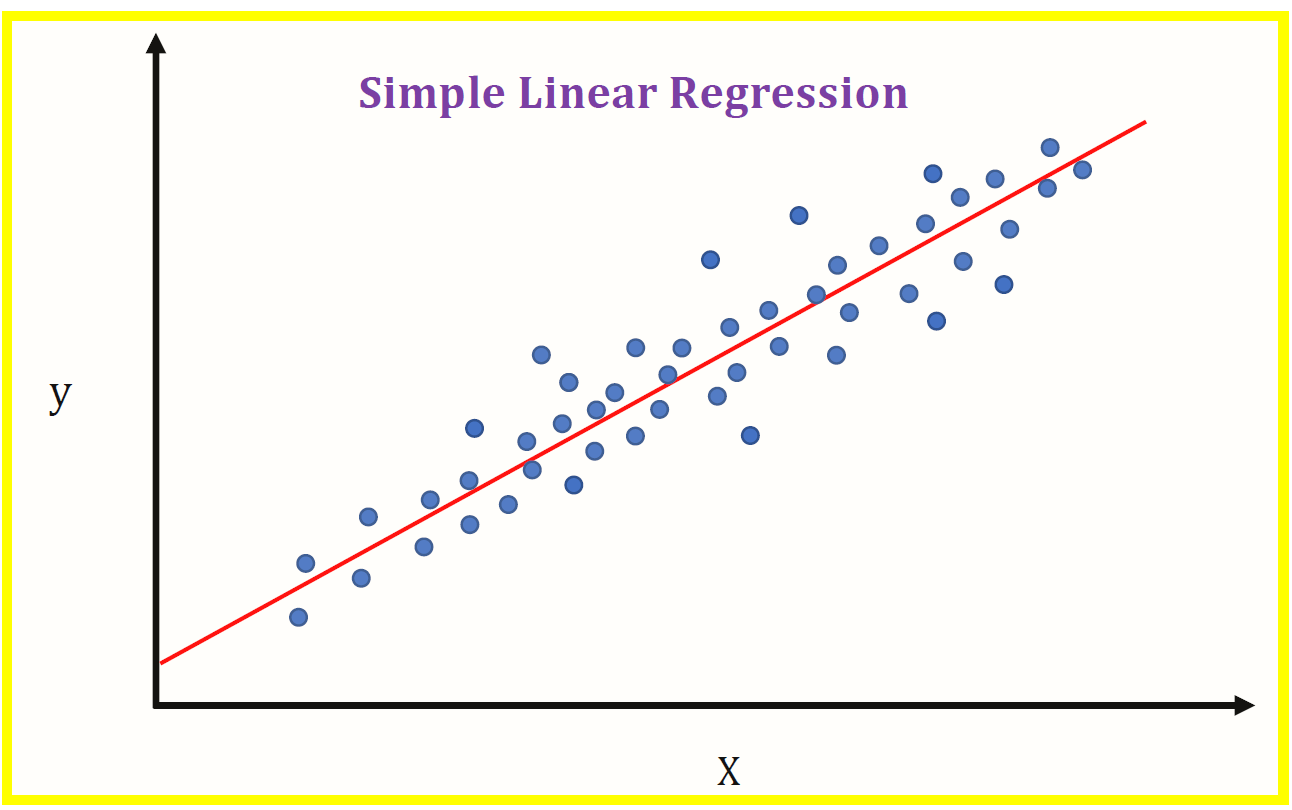
\includegraphics[width=0.8\textwidth]{images/linear-regression.png}
	\caption{Simple Linear Regression}
	\centering
	\label{label:file_name}
\end{figure}
In statistics, linear regression is a linear approach to modelling the relationship between a scalar response and one or more explanatory variables (also known as dependent and independent variables). The case of one explanatory variable is called simple linear regression; for more than one, the process is called multiple linear regression.\\
\\
Linear Regression is the first type of regression algorithm to be studied rigorously, and to be used extensively in practical applications as the models which depend linearly on their unknown parameters are easier to fit than models which are non-linearly related to their parameters.


\subsection*{Logistic Regression}
\addcontentsline{toc}{subsection}{Logistic Regression}
\begin{figure}[!ht]
	\centering
	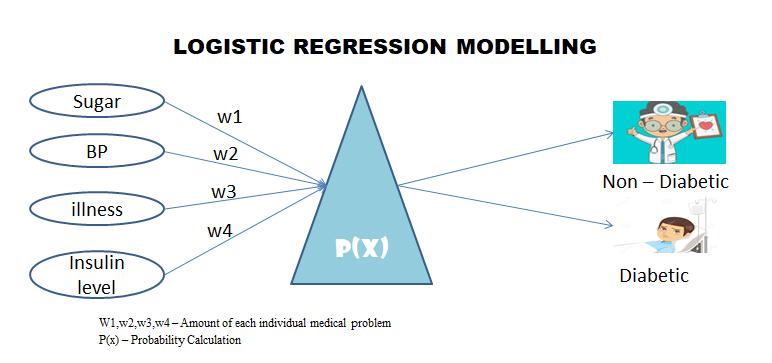
\includegraphics[width=0.8\textwidth]{images/logistic-regression.png}
	\caption{Logistic Regression Modelling}
	\centering
	\label{label:logistic}
\end{figure}
In statistics, the logistic model is used to model the probability of a certain class or event existing such as pass/fail, win/lose, alive/dead or healthy/sick. This can be extended to model several classes of events such as determining whether an image contains a cat, dog, lion, etc. Each object being detected in the image would be assigned a probability between 0 and 1, with a sum of one.\\
\\
It is named after the logistic function, also called the sigmoid function was developed by statisticians to describe properties of population growth in ecology, rising quickly and maxing out at the carrying capacity of the environment. It’s an S-shaped curve that can take any real-valued number and map it into a value between 0 and 1, but never exactly at those limits.


\subsection*{Decision Tree}
\addcontentsline{toc}{subsection}{Decision Tree}
\begin{figure}[!ht]
	\centering
	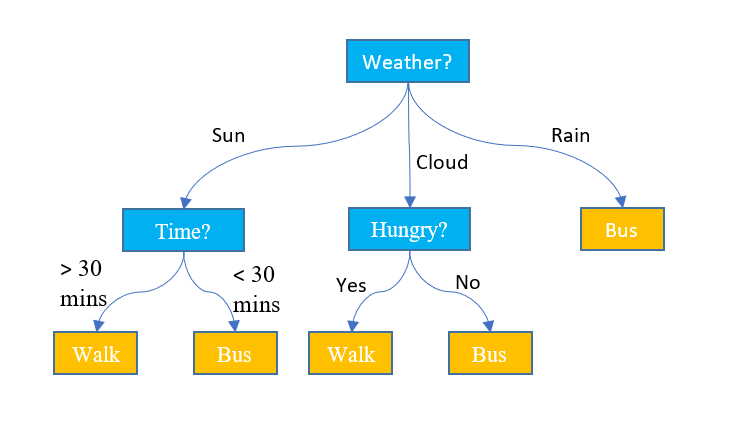
\includegraphics[width=0.8\textwidth]{images/decision-tree.png}
	\caption{Decision Tree example}
	\centering
	\label{label:decision-tree}
\end{figure}
In decision analysis, a decision tree can be used to visually and explicitly represent decisions and decision making. As the name goes, it uses a tree-like model of decisions. Though a commonly used tool in data mining for deriving a strategy to reach a particular goal, its also widely used in machine learning.\\
\\
Decision trees classify instances by sorting them down the tree from the root to some leaf node, which provides the classification of the instance. An instance is classified by starting at the root node of the tree, testing the attribute specified by this node, then moving down the tree branch corresponding to the value of the attribute. This process is then repeated for the subtree rooted at the new node.\\
Some Strengths of Decision tree approach are:
\begin{itemize}
    \item they are able to generate understandable rules.
    \item perform classification without requiring much computation.
    \item they are able to handle both continuous and categorical variables.
    \item they provide a clear indication of which fields are most important for prediction or classification.
\end{itemize}

Some of its weaknesses include:
\begin{itemize}
    \item they are less appropriate for estimation tasks where the goal is to predict the value of a continuous attribute.
    \item they are prone to errors in classification problems with many class and relatively small number of training examples.
    \item they can be computationally expensive to train.
\end{itemize}


\subsection*{Random Forest}
\addcontentsline{toc}{subsection}{Random Forest}
\begin{figure}[!ht]
	\centering
	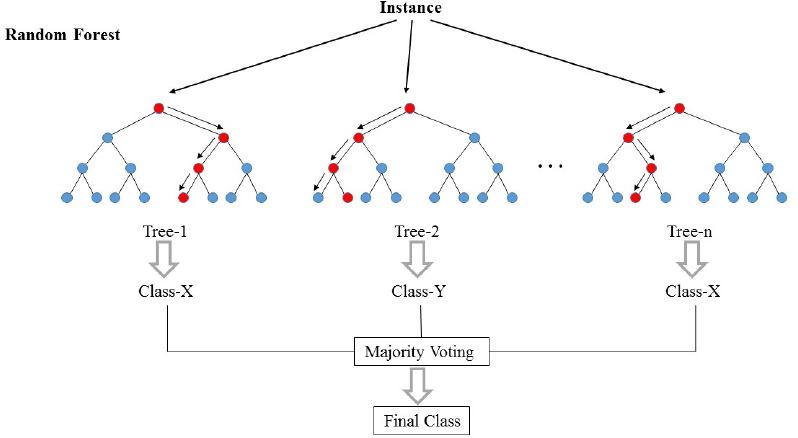
\includegraphics[width=0.8\textwidth]{images/random-forest.jpg}
	\caption{Random Forest Classification}
	\centering
	\label{label:randomforest}
\end{figure}
Random forests or random decision forests are an ensemble learning method for classification, regression and other tasks that operates by constructing a multitude of decision trees at training time.For classification tasks, the output of the random forest is the class selected by most trees. For regression tasks, the mean or average prediction of the individual trees is returned.\\
\\
Random decision forests correct for decision trees habit of overfitting to their training set. They generally outperform decision trees, however data characteristics can affect their performance. It adds additional randomness to the model, while growing the trees. Instead of searching for the most important feature while splitting a node, it searches for the best feature among a random subset of features. This results in a wide diversity that generally results in a better model.\\
\\
Random forests are frequently used as "blackbox" models in businesses, as they generate reasonable predictions across a wide range of data while requiring little configuration.

\subsection*{Bayes Classifier}
\addcontentsline{toc}{subsection}{Bayes Classifier}
In statistics, naive Bayes classifiers are a family of simple "probabilistic classifiers" based on applying Bayes' theorem with strong independence assumptions between the features. They are among the simplest Bayesian network models.\\
\\
They are among the simplest Bayesian network models. Despite their naive design and apparently oversimplified assumptions, naive Bayes classifiers have worked quite well in many complex real-world situations.\\
An advantage of naive Bayes is that it only requires a small number of training data to estimate the parameters necessary for classification.


\subsection*{K{-}Nearest Neighbors(KNN)}
\addcontentsline{toc}{subsection}{K{-}Nearest Neighbors}
\begin{figure}[!ht]
	\centering
	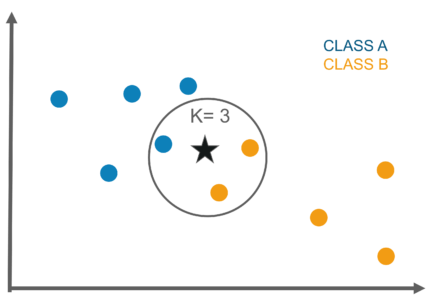
\includegraphics[width=0.8\textwidth]{images/knn.png}
	\caption{Classifying unknown example with K=3}
	\centering
	\label{label:knn}
\end{figure}
The k-nearest neighbors (KNN) algorithm is a simple, supervised machine learning algorithm that can be used to solve both classification and regression problems. It’s easy to implement and understand, but has a major drawback of becoming significantly slows as the size of that data in use grows.\\
\\
KNN works by finding the distances between a query and all the examples in the data, selecting the specified number examples (K) closest to the query, then votes for the most frequent label (in the case of classification) or averages the labels (in the case of regression).


\subsection*{Support Vector Machines(SVM)}
\addcontentsline{toc}{subsection}{Support Vector Machines}
\begin{figure}[!ht]
	\centering
	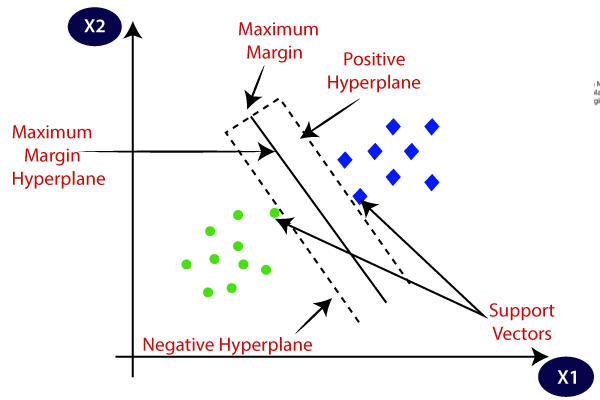
\includegraphics[width=0.8\textwidth]{images/svm.png}
	\caption{Support Vector Machine example}
	\centering
	\label{label:svm}
\end{figure}
“Support Vector Machine” (SVM) is a supervised machine learning algorithm which can be used for both classification or regression challenges. However,  it is mostly used in classification problems. In the SVM algorithm, we plot each data item as a point in n{-}dimensional space (where n is number of features you have) with the value of each feature being the value of a particular coordinate. Then, we perform classification by finding the hyper-plane that differentiates the two classes.\\
\\
Hyperplanes are decision boundaries that help classify the data points. Data points falling on either side of the hyperplane can be attributed to different classes. Also, the dimension of the hyperplane depends upon the number of features. If the number of input features has dimension n, then the hyperplane will be a (n-1) dimensional affine plane.\\
\\
Support Vectors are simply the co-ordinates of individual observation. The SVM classifier is a frontier which best segregates the two classes (hyper-plane/ line).

\end{document}

%-------------------------------------------------------------------------------
% SNIPPETS
%-------------------------------------------------------------------------------

%\begin{figure}[!ht]
%	\centering
%	\includegraphics[width=0.8\textwidth]{file_name}
%	\caption{}
%	\centering
%	\label{label:file_name}
%\end{figure}

%\begin{figure}[!ht]
%	\centering
%	\includegraphics[width=0.8\textwidth]{graph}
%	\caption{Blood pressure ranges and associated level of hypertension (American Heart Association, 2013).}
%	\centering
%	\label{label:graph}
%\end{figure}

%\begin{wrapfigure}{r}{0.30\textwidth}
%	\vspace{-40pt}
%	\begin{center}
%		\includegraphics[width=0.29\textwidth]{file_name}
%	\end{center}
%	\vspace{-20pt}
%	\caption{}
%	\label{label:file_name}
%\end{wrapfigure}

%\begin{wrapfigure}{r}{0.45\textwidth}
%	\begin{center}
%		\includegraphics[width=0.29\textwidth]{manometer}
%	\end{center}
%	\caption{Aneroid sphygmomanometer with stethoscope (Medicalexpo, 2012).}
%	\label{label:manometer}
%\end{wrapfigure}

%\begin{table}[!ht]\footnotesize
%	\centering
%	\begin{tabular}{cccccc}
%	\toprule
%	\multicolumn{2}{c} {Pearson's correlation test} & \multicolumn{4}{c} {Independent t-test} \\
%	\midrule	
%	\multicolumn{2}{c} {Gender} & \multicolumn{2}{c} {Activity level} & \multicolumn{2}{c} {Gender} \\
%	\midrule
%	Males & Females & 1st level & 6th level & Males & Females \\
%	\midrule
%	\multicolumn{2}{c} {BMI vs. SP} & \multicolumn{2}{c} {Systolic pressure} & \multicolumn{2}{c} {Systolic Pressure} \\
%	\multicolumn{2}{c} {BMI vs. DP} & \multicolumn{2}{c} {Diastolic pressure} & \multicolumn{2}{c} {Diastolic pressure} \\
%	\multicolumn{2}{c} {BMI vs. MAP} & \multicolumn{2}{c} {MAP} & \multicolumn{2}{c} {MAP} \\
%	\multicolumn{2}{c} {W:H ratio vs. SP} & \multicolumn{2}{c} {BMI} & \multicolumn{2}{c} {BMI} \\
%	\multicolumn{2}{c} {W:H ratio vs. DP} & \multicolumn{2}{c} {W:H ratio} & \multicolumn{2}{c} {W:H ratio} \\
%	\multicolumn{2}{c} {W:H ratio vs. MAP} & \multicolumn{2}{c} {\% Body fat} & \multicolumn{2}{c} {\% Body fat} \\
%	\multicolumn{2}{c} {} & \multicolumn{2}{c} {Height} & \multicolumn{2}{c} {Height} \\
%	\multicolumn{2}{c} {} & \multicolumn{2}{c} {Weight} & \multicolumn{2}{c} {Weight} \\
%	\multicolumn{2}{c} {} & \multicolumn{2}{c} {Heart rate} & \multicolumn{2}{c} {Heart rate} \\
%	\bottomrule
%	\end{tabular}
%	\caption{Parameters that were analysed and related statistical test performed for current study. BMI - body mass index; SP - systolic pressure; DP - diastolic pressure; MAP - mean arterial pressure; W:H ratio - waist to hip ratio.}
%	\label{label:tests}
%\end{table}